A digital reverb effect was chosen as a natural complement to the pitch shifting functionality of the module. 
Reverberation widens the sonic palette of the sampler significantly: 
by pushing parameters to extremes, the effect can produce sounds ranging from harsh metallic resonances to wide, lush, long-lasting spatial decay -- far beyond conventional room simulation.

\subsection{Problem Statement}

The central challenge is implementing a perceptually plausible, \textit{flexible} reverb on microcontroller-class hardware, where computational resources and memory are strictly limited. 
A reverb algorithm is required that is both computationally lightweight and perceptually convincing, while exposing a set of parameters for real-time RT60 control, room size and wet mix amount.


Room simulation can become very complex when attempting to physically model the acoustic behaviour of a space. Important aspects include correct physical behaviour of sound waves, perceptually convincing reverberation, and early and late reflection simulation. \cite[pp.~87-95]{juliuso.smithPhysicalSignalProcessing}

All of these are relevant considerations, but implementing each in depth is out of scope for this project, as the reverb is merely the DSP component of a larger system. 
The goal is a straightforward implementation that demonstrates the real-time capabilities of the hardware while producing aesthetically interesting spatial effects. 
For this reason, one of the earliest concepts of artificial reverberation based on discrete-time signal processing was chosen -- constructed by Schroeder in the early 1960s and known as the \textit{Schroeder Reverberator}.

\subsection{Theory of the Schroeder Reverb}
% Schroeder structure, why prime delays, what RT60 is.

Schroeders original proposal is a combination of \textit{comb} and \textit{allpass} filters. \cite{m.r.schroederJournalAudioEngineering1962}[pp.~219-223]
The implementation structure used in this project includes a bank of parallel comb filters, combining into a series of allpass filters.
%The variant used here -- including lowpass-feedback comb filters -- is also known as the \textbf{Moore} variant of the reverberator.

\begin{figure}[htbp]
	\centering
	\vspace{-2em}
	\makebox[\textwidth][c]{%
		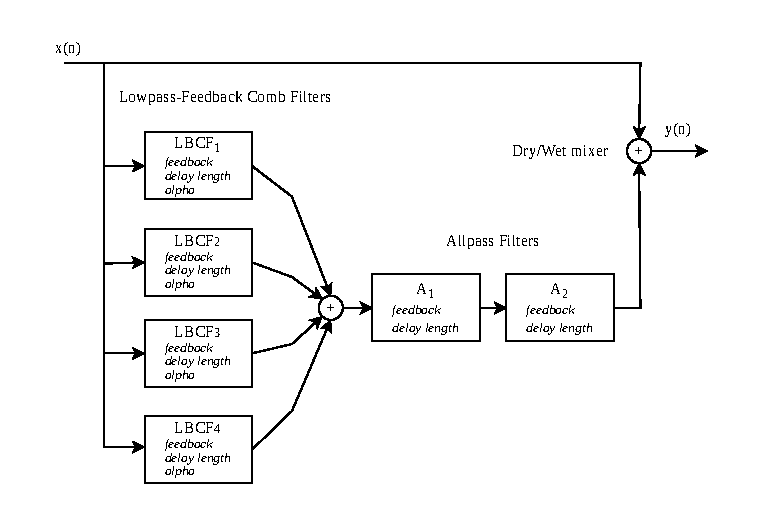
\includegraphics[width=0.8\textwidth]{../images/schroeder_reverb/schroeder_reverb.drawio.pdf}
	}
	\vspace{-2em}
	\caption{Schroeder Reverb Block Diagram}
	\label{fig:schroeder_block}
\end{figure}

Figure \ref{fig:schroeder_block} shows the basic structure of the implemented reverb.
Cursive parameters, such as filter coefficient \textit{alpha}, the \textit{feedback} gain and \textit{delay length}, are implemented as controllable by outside of the component.

The combination of parallel comb filters feeding into series allpass filters is a psychoacoustically motivated design. 
The comb filters produce the characteristic frequency-domain coloration and exponential decay of a reverberant space, but their echo density is too sparse on its own. 
The allpass filters, also called \textit{diffusers}, increase the echo density without adding frequency coloration, since their magnitude response is flat across all frequencies. 
Together, the structure achieves both a perceptually convincing decay envelope and a sufficiently dense late reverberation tail. \cite[p.~97]{juliuso.smithPhysicalSignalProcessing}

\subsubsection{Feedback Comb Filter}
\label{sec:comb_filter}

At the basis of the \textit{Schroeder Reverberator} is a structure of parallel comb filters.
Comb filters are fundamental building blocks for digital audio effects. 
Its most obvious example is a simple echo implementation \cite[p.~57]{juliuso.smithPhysicalSignalProcessing}.

The most simple variant is a \textit{feedforward} comb filter. It takes the input signal $x[n]$ and adds a delayed copy, shifted by $D$ samples, to produce the output $y[n]$. Since the delayed signal is not fed back into the input, each reflection occurs only once.

In theory, a room reverberation simulation can be constructed using only \textit{feedforward} 
comb filters, where each reflection is modelled by a separate filter instance. 
In practice however, this becomes computationally expensive for a convincing 
reverb with many reflections.~\cite[p.~85]{juliuso.smithPhysicalSignalProcessing}

\begin{figure}[H] \vspace{-1em} \centering \makebox[\textwidth][c]{ 			
	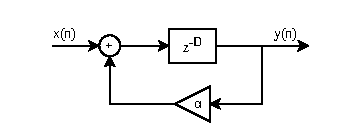
\includegraphics[width=0.5\textwidth]{../images/schroeder_reverb/comb.drawio.pdf}} 
	\vspace{-2em} 
	\caption{Feedback Comb Filter}  
	\label{fig:schroeder_comb} 
\end{figure}


Where the \textit{feedforward} comb filter implements an FIR filter, the \textit{feedback} comb filter (Figure \ref{fig:schroeder_comb}) takes the delayed output and feeds it back to the input. This filter type is also known as an IIR (Infinite Impulse Response) or \textit{recursive} filter, and is described by the difference equation:
\begin{equation}
y[n] = x[n] + \alpha \cdot y[n - D]
\end{equation}
where $\alpha$ is the feedback gain and $D$ the delay in samples.

The feedback comb filter can be understood as a physical model of a series of 
exponentially decaying echoes, resembling a signal reflecting between two parallel 
walls. For this reason, feedback comb filters are preferred in reverb design, 
offering a more natural decay while remaining computationally 
efficient. \cite[p.~98]{juliuso.smithPhysicalSignalProcessing}

\begin{wrapfigure}{r}{0.57\textwidth}
	\centering
	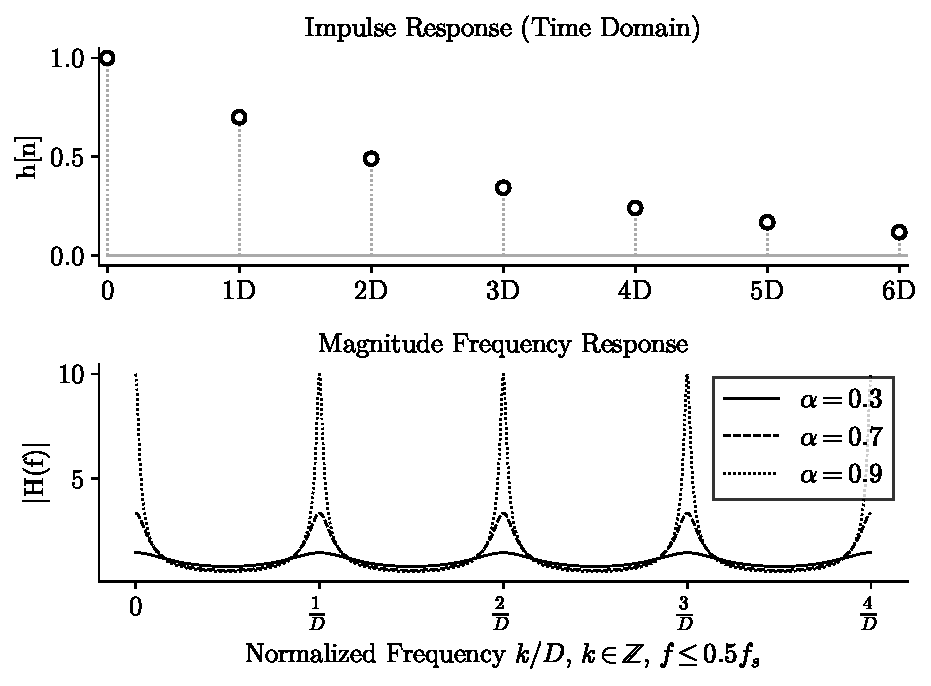
\includegraphics[width=0.54\textwidth]{../images/schroeder_reverb/fig_comb_filter_response.pdf}
	\caption{Impulse and Frequency Response of Feedback Comb Filter with different feedback gain $\alpha$}
	\label{fig:schroeder_comb_filter_response}
\end{wrapfigure}

The feedback coefficient $\alpha$ must be less than 1 in magnitude for the filter to be stable. 
Otherwise each echo would be louder than the previous one, causing the output to diverge and become unstable.

A feedback gain close to $1$ produces a very slowly decaying tail, which can be an interesting
artistic effect but must be used with caution. 

In Figure~\ref{fig:schroeder_comb_filter_response} the decaying echoes at uniform intervals of
$D$ samples are clearly visible in the impulse response.
The characteristic frequency response resembling a comb gives the filter its name.
The evenly spaced peaks arise because constructive interference occurs at every integer multiple
of $f_s/D$, producing resonances separated by $1/D$ in normalized frequency.

Essentially the peaks are frequencies where the delay $D$ is an exact multiple of the period of that frequency. 
The delayed copy arrives back perfectly in phase with 
the new input, and they reinforce each other. At the troughs, the input signal is exactly \textit{out of phase} with the fed-back delayed signal, causing cancellation.

\paragraph{Lowpass-Feedback Comb Filter}

Instead of using a standard feedback comb filter, this project employs a \textit{lowpass-feedback} comb filter (\ac{LBCF}), which places a filter $H_f(z)$ in the feedback path alongside the feedback gain $\alpha$.

\begin{figure}[H]
	\centering
	\vspace{-1.5em}
	\makebox[\textwidth][c]{%
		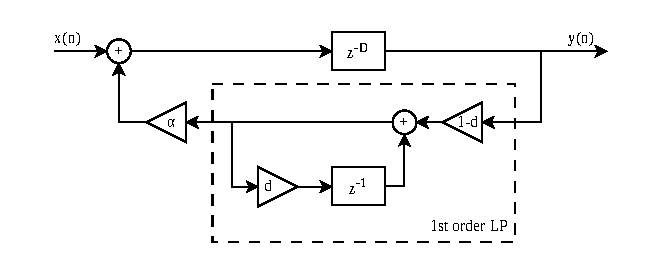
\includegraphics[width=0.7\textwidth]{../images/schroeder_reverb/lp_filtered_comb.drawio.pdf}
	}
	\vspace{-2.0em}
	\caption{Filtered-Feedback Comb Filter with 1st order Lowpass}
	\label{fig:schroeder_lbcf}
\end{figure}

The transfer function in the $z$-domain is given by:

\begin{equation}
	H_{LBCF}(z) = \frac{z^{-D}}{1 - \alpha \cdot H_{f}(z) \cdot  z^{-D}}
\end{equation}

Note that the transfer function is given here with the output taken after the delay, differing slightly from the notation in \cite{juliuso.smithPhysicalSignalProcessing}.
 
Using a first-order lowpass $H_f(z) = H_{lp}(z)$ with a damping coefficient $d$:
\begin{equation}
	H_{lp}(z) = \frac{1 - d}{1 - d \cdot z^{-1}}
\end{equation}

the full transfer function becomes:

\begin{equation}
H_{LBCF}(z) = \frac{z^{-D}}{1 - \alpha \frac{1 - d}{1 - d \cdot z^{-1}}  z^{-D}}
\end{equation}

The effect of the lowpass in the feedback path causes high frequencies to decay faster than low frequencies, producing a more natural reverb tail. 
Adding a low-pass filter in the feedback loop can effectively recreate the losses that happen when a signal travels back and forth between two places, as happens in real rooms. \cite[p.~62]{juliuso.smithPhysicalSignalProcessing}


\begin{wrapfigure}{r}{0.57\textwidth}
	\centering
	\vspace{-2.0em}
	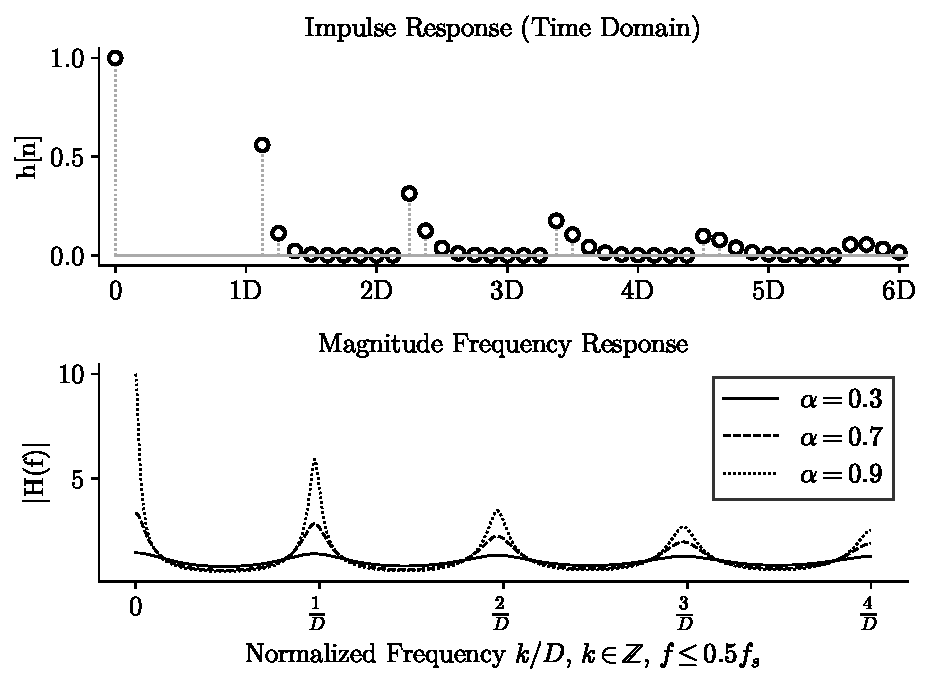
\includegraphics[width=0.55\textwidth]{../images/schroeder_reverb/fig_comb_filter_lp_feedback_response.pdf}
	\caption{Impulse and Frequency Response of Lowpass Feedback Comb Filter with different feedback gain $\alpha$ and filter coefficient $d=0.2$}
	\label{fig:schroeder_comb_filter_lp_feedback_response}
\end{wrapfigure}

\paragraph{Impulse and Frequency Response} 
In Figure~\ref{fig:schroeder_comb_filter_lp_feedback_response}, the effect of the lowpass filter in the feedback path is clearly visible. 

Compared to the pure feedback comb filter in Figure \ref{fig:schroeder_comb_filter_response}, the impulse response shows non-zero samples between the echo peaks, caused by the smearing effect of the one-pole IIR filter.

In the frequency response, the comb peaks are attenuated at higher frequencies, as the lowpass reduces the feedback gain progressively with frequency, resulting in shorter decay times for high frequencies than for low frequencies.

\clearpage
\subsubsection{Allpass Filter}

The allpass filter passes all frequencies at equal gain. 
Unlike lowpass or highpass filters, it does not attenuate any frequency band. 
Instead, it affects only the \textit{phase} of the signal, introducing frequency-dependent delays while leaving the magnitude response flat at unity gain across all frequencies. 
In the context of the Schroeder reverberator, allpass filters are used as \textit{diffusers}: they increase the echo density of the late reverberation without coloring the sound, complementing the tonal decay provided by the comb filter bank. \cite{juliuso.smithPhysicalSignalProcessing}

\begin{figure}[H]
	\centering
	\makebox[\textwidth][c]{%
		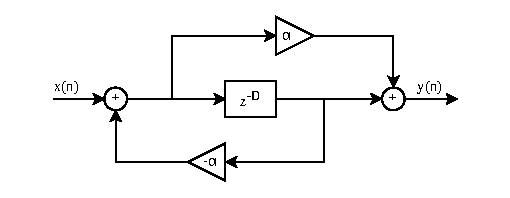
\includegraphics[width=0.6\textwidth]{../images/schroeder_reverb/allpass.drawio.pdf}
	}
	\caption{Allpass Filter}
	\label{fig:schroeder_allpass}
\end{figure}

The allpass filter can be constructed by cascading a \textit{feedforward} and \textit{feedback} comb filter delay line (see Section \ref{sec:comb_filter}). Figure \ref{fig:schroeder_allpass} illustrates the combination of the two comb filter variants. \cite[p.69]{juliuso.smithPhysicalSignalProcessing}
 \\

When inspecting the transfer function:
\begin{equation}
	H(z) = \frac{\alpha + z^{-D}}{1 + \alpha z^{-D}}
\end{equation}

It becomes clear, how the Schroeder allpass works. The numerator and denominator of $H(z)$ are mirror images of each other. 

\vspace{2.0em}

\begin{wrapfigure}{r}{0.57\textwidth}
	\centering
	\vspace{-2.0em}
	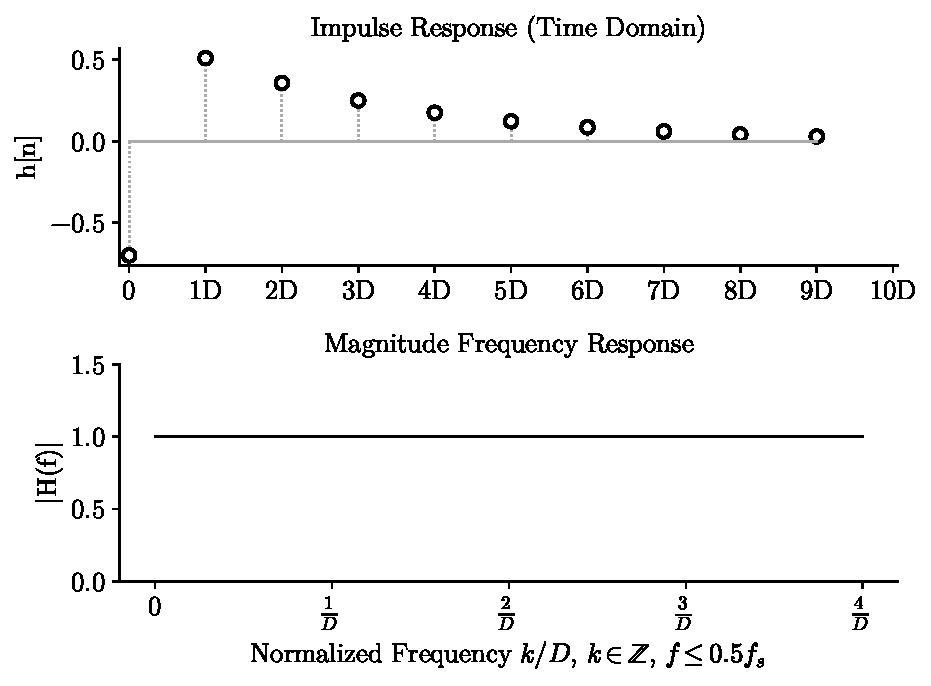
\includegraphics[width=0.55\textwidth]{../images/schroeder_reverb/fig_allpass_response.pdf}
	\caption{Impulse and Frequency Response of Allpass Filter}
	\label{fig:schroeder_allpass_filter_response}
\end{wrapfigure}


Whatever the feedback amplifies at a certain frequency, the feedforward cancels exactly, leaving only a phase shift (the delay in time-domain) behind.  
This causes the totally flat frequency response of the \textit{allpass} filter.
Note the similar impulse response to the feedback comb filter \ref{fig:schroeder_comb_filter_response}

\clearpage
\subsection{Design and Implementation}
% 4-comb + 2-allpass, LP damping in comb feedback path, prime stereo decorrelation.

The implemented reverberator follows a simplified variant of the \textit{Freeverb} \cite{freeverb-github} variant of the Schroeder structure -- a public-domain C++ program, used extensively in the free-software community -- adapted here for embedded C on a microcontroller target. 

It consists of four parallel lowpass-feedback comb filters summing into two series allpass filters, per channel \cite[p.~101]{juliuso.smithPhysicalSignalProcessing}. The full z-domain block diagram is shown in Figure~\ref{fig:schroeder_block_detailed}.

\begin{figure}[htbp]
	\centering
	\vspace{-1.1em}
	\makebox[\textwidth][c]{
		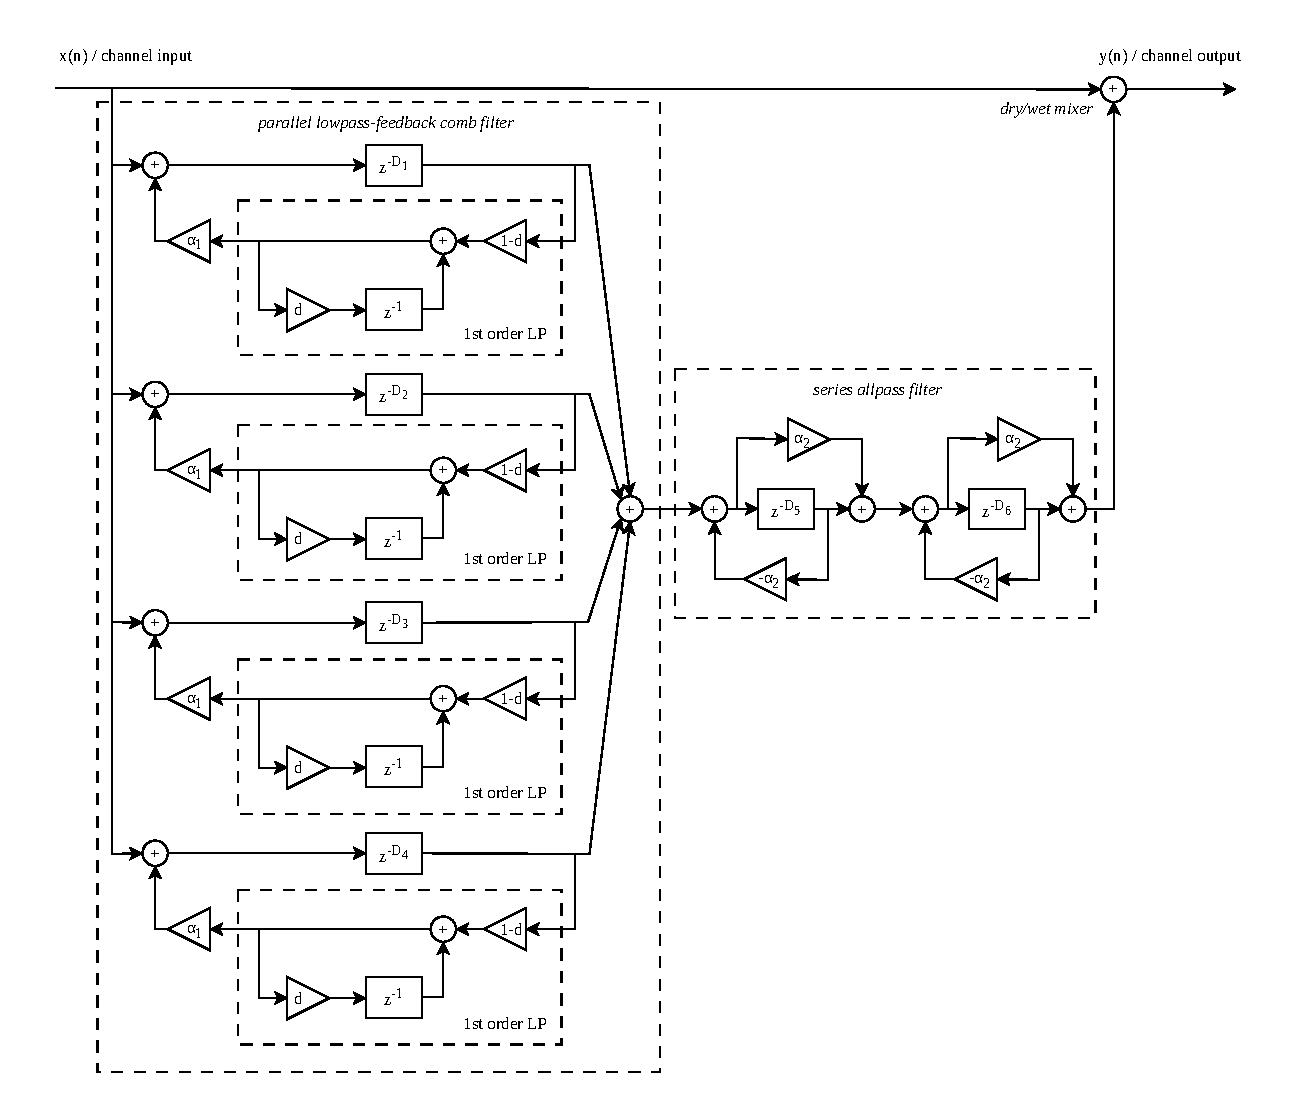
\includegraphics[width=1.1\textwidth]{../images/schroeder_reverb/schroeder_reverb_block_detailed.drawio.pdf}	
		}
	\vspace{-2.0em}
	\caption{Schroeder Reverb Block Diagram}
	\label{fig:schroeder_block_detailed}
\end{figure}

\vspace{-2.0em}

\paragraph{Delay Line Structure} Each filter (comb or allpass) is backed by a statically allocated circular float buffer that holds the sample history required by the delay line. 
Both filters share the same \texttt{sr\_delay\_t} struct, which stores the buffer pointer, its maximum allocated \texttt{size}, the currently active \texttt{length}, and a write index \texttt{idx}. 
Separating \texttt{size} from \texttt{length} allows the active delay time to be changed at runtime without reallocating memory. 
The struct also carries filter-specific state: \texttt{feedback} gain and \texttt{lp\_state} for the comb filter's damped feedback path.

\begin{listing}[H]
\begin{minted}{c}
typedef struct {
	float feedback;
	float* buf;
	uint32_t size;   /**< Buffer capacity in samples. */
	uint32_t idx;
	uint16_t length; /**< Active delay length in samples (<= size). */
	
	float lp_state;
	float lp_alpha;  /**< One-pole LP coefficient in the comb feedback path. */
} sr_delay_t;
\end{minted}
\vspace{-2.0em}
\caption{delay-line struct type definition}
\label{lst:schroeder-delayline-struct}
\end{listing}

\vspace{-2.5mm}	
The functionality of both, the comb- and allpass filters are implemented in the respective \texttt{*\_process} functions:

\begin{listing}[H]
\vspace{-2.5mm}	
\begin{minted}[linenos]{c}
static float comb_process(sr_delay_t* d, float in) {
	// calculate read index with wraparound depending on set .length parameter
	uint32_t read_idx = (d->idx + d->size - d->length) % d->size;
	float y = d->buf[read_idx];
	
	float feedback_signal = y * d->feedback;
	
	// one-pole lowpass on each combs fb path.
	d->lp_state = (1.0f - d->lp_alpha) * feedback_signal + d->lp_alpha * d->lp_state;
	d->buf[d->idx] = in + d->lp_state;
	
	d->idx++;
	if (d->idx >= d->size)
	d->idx = 0;
	
	return y;
}

static float allpass_process(sr_delay_t* d, float in) {
	// calculate read index with wraparound depending on set .length parameter
	uint32_t read_idx = (d->idx + d->size - d->length) % d->size;
	float buf = d->buf[read_idx];
	
	float y = -in + buf;
	d->buf[d->idx] = in + buf * d->feedback;
	
	d->idx++;
	if (d->idx >= d->size)
	d->idx = 0;
	
	return y;
}
\end{minted}
\vspace{-2.0em}
\caption{process functions of comb and allpass filters}
\label{lst:schroeder-process-functions}
\end{listing}


Both underlying \texttt{sr\_delay\_t} structures share the same ring buffer mechanics: \texttt{idx} advances by one each tick, and the delay tap is read from \mintinline{c}|(idx + size - length) % size|, placing it exactly \texttt{length} samples behind the write head in O(1) without branching.

The comb filter runs the feedback sample through a one-pole lowpass (line 9) before writing it back with the input (line 10), implementing damped feedback in-place. 
The allpass uses the same ring structure but applies the Schroeder topology (lines 22--25) directly, yielding flat magnitude response with phase dispersion.

\paragraph{Static Memory Allocation} 
\label{sec:schroeder_memory_allocation}

Twelve buffers are allocated in total: eight comb buffers of \texttt{MAX\_COMB\_LEN}~=~1620 samples and four allpass buffers of \texttt{MAX\_AP\_LEN} = 600 samples. At 32-bit float precision (4 bytes per sample), the total static memory footprint is:
\begin{equation}
(8 \times 1620 + 4 \times 600) \times 4\ \text{bytes} = 61.4\ \text{kB}
\end{equation}

The buffer size and thus the maximum delay lengths are directly correlated to the maximum room size of the algorithm. 
Increasing the base delay lengths would produce a larger perceived space at \texttt{size = 1}, at the cost of higher memory consumption. 
%The current values were chosen to provide an aesthetically pleasing maximum room size while maintaining a conservative memory footprint, preserving available RAM for the sample playback buffers in the system.

\paragraph{Delay Length Selection} Using mutually prime delay line lengths, i.e. values sharing no common factors, helps avoid spectral clustering and unnatural resonances in the frequency response. 
When delay lengths share common factors, their resonant frequencies align, causing certain frequencies to be disproportionately reinforced. By choosing mutually prime lengths, the resonances are maximally spread across the spectrum, resulting in a evenly decay envelope.
The delay lengths were selected empirically by ear from prime numbers, starting from a base set and scaled by a room size parameter. 
The comb delays (30--34\,ms) target the late reverberation tail, while the allpass delays are kept short (5--12\,ms) to increase echo density without introducing perceivable discrete echoes. 
The chosen base delay lengths are:

\begin{table}[H]
    \centering
    \begin{tabular}{lcccc}
        \hline
        & \multicolumn{4}{c}{Comb Filter Delays (samples)} \\
        & 1 & 2 & 3 & 4 \\
        \hline
        Left  & 1553 & 1613 & 1499 & 1427 \\
        Right & 1567 & 1601 & 1487 & 1433 \\
        \hline
    \end{tabular}
    \hspace{2em}
    \begin{tabular}{lcc}
        \hline
        & \multicolumn{2}{c}{Allpass Delays (samples)} \\
        & 1 & 2 \\
        \hline
        Left  & 223 & 557 \\
        Right & 229 & 563 \\
        \hline
    \end{tabular}
    \caption{Base delay line lengths for comb and allpass filters (in samples at \qty{48}{\kilo\hertz}).}
    \label{tab:delay-lengths}
\end{table}

The slight asymmetry between left and right channels provides stereo decorrelation, widening the perceived sound field without additional processing.

\paragraph{Stability and Feedback Scaling} To prevent instability as the room size parameter is reduced, the feedback gain is scaled automatically using two macros:

\begin{verbatim}
	#define COMB_FEEDBACK(size)   (0.97f + 0.01f * (1.0f - size))
	#define ALLPASS_FEEDBACK(size)(0.68f + 0.01f * (1.0f - size))
\end{verbatim}

As the room size decreases, delay lines shorten and the filter accumulates energy more rapidly. 
The macros compensate by slightly increasing the base feedback value as size decreases, maintaining a perceptually consistent decay across the full parameter range. 
The feedback value passed in by the user is additionally clamped to $[0,0.999]$ before being applied, ensuring the filter never reaches the instability threshold of $\alpha = 1$. 
A minimum room size of 0.30 is enforced to prevent the delay lines from becoming so short that the filter becomes difficult to stabilise.

\paragraph{Controllable Parameters}
\begin{center}
    \small
    \begin{tabular}{ll}
        \toprule
        \textbf{Parameter} & \textbf{Description} \\
        \midrule
        \texttt{wet}            & Dry/wet balance; $\texttt{dry} = 1 - \texttt{wet}$ enforced automatically. \\
        \texttt{feedback} $(\alpha)$ & RT60 decay time; routed through stability macros to compensate for room size. \\
        \texttt{size}           & Uniformly scales all delay lengths, preserving prime relationships. \\
        \texttt{lp\_alpha} $(d)$  & One-pole IIR cutoff in each comb path; attenuates highs for natural decay. \\
        \bottomrule
    \end{tabular}
\end{center}

\paragraph{Parameter Coupling}
\label{sec:schroeder_parameter_coupling}
The feedback gain and room size parameters are implicitly coupled through the stability macros. The \texttt{size} scalar is stored in the \texttt{schroeder\_stereo\_t} struct so that \\ \texttt{schroeder\_rev\_set\_feedback} can reference it when computing the scaled feedback values:
\begin{minted}{c}
	float comb_fb = feedback * COMB_FEEDBACK(rev->size);
\end{minted}